\section{簡介}
在上一章中,我們嘗試了使用聲學組型加強語意檢索的成果,使得系統能夠在接收到文字形式的查詢詞後,進行語意檢索回傳給使用者語意相關的語音文件。這樣的框架需要使用者在每次查詢詞都要對系統輸入文字形式的查詢詞,但是對使用者來說,使用口語形式的輸入才是最自然的輸入方法,尤其在行動裝置與穿戴式裝置日益盛行的情況下,如果能讓使用者不需要使用行動裝置的鍵盤就進行檢索,將能大幅提高使用者體驗與使用者的滿意度。另一方面,如果使用者輸入的是口語形式的查詢詞,那系統就能直接使用語音去直接檢索語音數位內容,如此就能直接在語音訊號上進行比對,這樣一來就能略過許多使用自動語音辨識系統 (ASR) 的困難:如辨識錯誤,辭典外詞彙等辨識困難,或是很難訓練一套好的聲學/語言模型與辭典,因為自動語音辨識系統的訓練過程需要很多人標注過的檔案,而這會導致這個訓練過程十分地昂貴,因此,在本章提出的架構中希望不用使用自動語音辨識系統。

本章的目標是達成「非監督式的語音內容語意檢索」,在這個狀況下,使用者輸入口語形式的查詢詞,系統直接進行語意檢索並回傳給使用者檢索結果,但如果沒有使用自動語音辨識系統,通常是很難實作語意檢索的,因為系統需要知道這些文字之間的關係才能進行語意檢索,這也是為什麼過去幾乎所有的非監督式檢索方法都只實作在口述語彙偵測
(系統只回傳包含查詢詞的文件),而沒有實作在語意檢索之中。但本章試圖使用之前提到的自動習得之聲學組型解決這個問題:系統先將所有語音文件轉寫成聲學組型序列,當使用者口述一段查詢詞給系統後,系統會使用動態時間校準 (Dynamic Time Warping, DTW) 直接在語音訊號上比對相似性,並按照語音文件中是否有出現此段查詢詞排序後產生第一次檢索結果,並假設第一次檢索結果的前 $N$
篇為虛擬相關文件,再將虛擬相關文件中很常一起出現的聲學組型當作和查詢詞語意相關的詞彙並將其當作新的查詢詞模型。如此一來,雖然系統沒辦法將語音文件轉寫成文字,但是系統仍然可以藉由其在聲學組型上的關聯性進行查詢詞擴展,並在查詢詞擴展的過程中找到與查詢詞語意相關的聲學組型,進而達成語意檢索的目的。

\section{基於聲學組型之語意檢索}
\subsection{系統架構}
系統架構如圖 ~\ref{fig:chap4_system},圖中的下半部為離線處理 (Offline Processing) 的部分,包括聲學組型的聲學模型、語言模型、辭典都是離線的時候自動從語料庫中學習出來的~\cite{chung2013unsupervised},有了聲學、語言模型和辭典後,即可用其建造出一個辨識系統 (圖~\ref{fig:chap4_system}中左下角) 將語音文件辨識成聲學組型形式的唯一最佳序列。圖~\ref{fig:chap4_system}中的上半部為在線處理 (Online Processing)
的部分,當使用者「口述」了一段查詢詞後,系統會使用片段式動態時間校準 (在圖~\ref{fig:chap4_system}中的檢索引擎1) 產生第一次檢索結果,並假設其中最相關的前 $N$ 篇為虛擬相關,虛擬相關文件中時常出現的聲學組型即可視作是與查詢詞語意相關的聲學組型,這些即為擴展後的查詢詞模型,接下來圖中的檢索引擎2 會利用擴展後查詢詞模型尋找之前得到的聲學組型形式的唯一最佳序列,如果這些唯一最佳序列中包含了這些與查詢詞語意相關的聲學組型,即是與原查詢詞語意相關的文件。

\begin{figure}
\centering
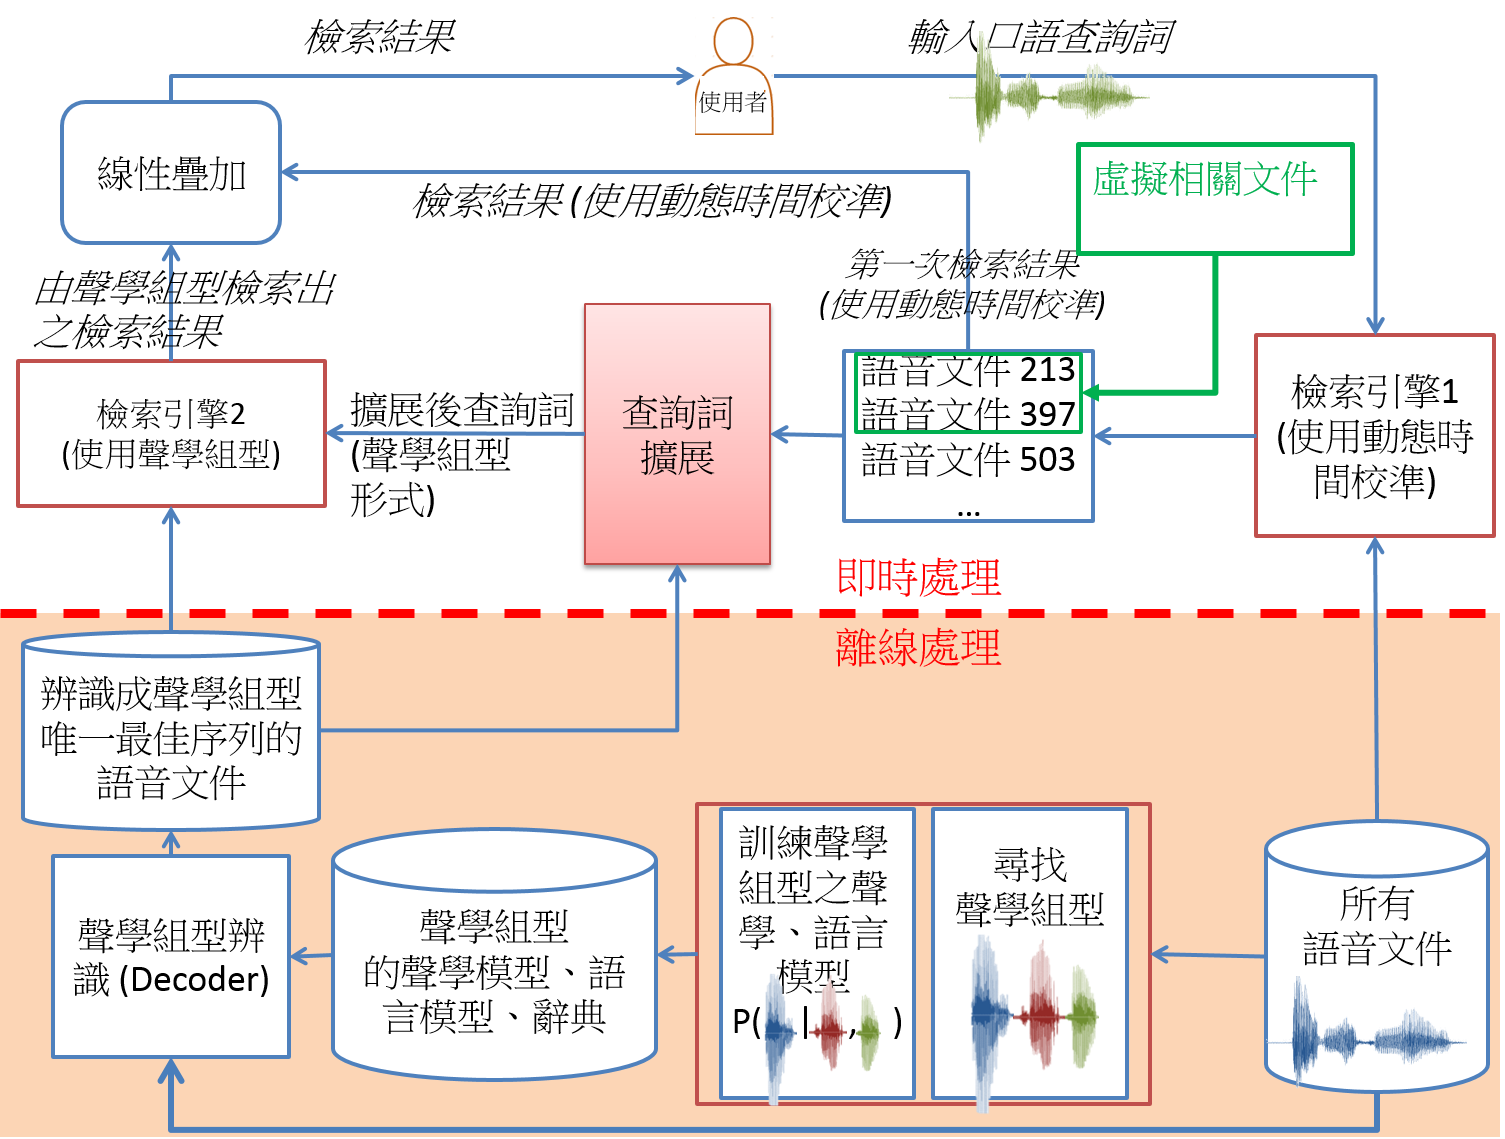
\includegraphics[scale=0.5]{images/chap4_system_zh.png}
\caption{系統架構示意圖} \label{fig:chap4_system}
\end{figure}

\subsection{前處理}
\subsubsection{聲學組型語言模型}
\label{sec:chap3_apd}
聲學組型指的是在某個特定語料中時常重複出現的聲音,比如像中文的音節、字等單位,這些聲學組型可以被用在口述文件分類、口述語彙偵測、語音文件檢索等。這裡使用的是本實驗室過去提出的雙層式聲學組型 (Two-Level Acoustic Pattern)~\cite{chung2013unsupervised} (細節列於 ~\ref{sec:chap2_ap}),其中包含了類詞的聲學組型 (類詞聲學組型是由數個類次詞聲學組型所組成)和類次詞的聲學組型、類詞聲學組型如何由類次詞聲學組型組合而成的辭典、類詞聲學組型的$N$連語言模型 (N-gram Language
Model)。每個類次詞聲學組型就是一個隱藏式馬可夫模型,所有的隱藏式馬可夫模型的參數、類次詞聲學組型的數目、類詞聲學組型的數目和類詞聲學組型的$N$連語言模型都是在非監督式的狀況下自動地從語料庫學習出來的。學習出聲學組型以後,這些聲學模型、語言模型和辭典可以用來建立一個辨識系統,並將這些語音文件辨識成聲學組型的序列,如此即可將語音文件$x$表示成聲學組型的語言模型$\phi_x$:

\begin{equation}
P(v|\phi_x) = \frac{C(v, x)}{\sum_v C(v, x)}
\end{equation}

$C(v, x)$ 為聲學組型$v$在語音文件$x$中出現的次數。$\phi_x$會再與聲學組型背景語言模型$\phi_b$做平滑化(即線性疊加),平滑化的語音文件模型為$\bar{\phi}_x$。$\phi_b$表示如下:

\begin{equation}
P(v|\phi_b) = \frac{\sum_{x\in C} C(v, x)}{\sum_v\sum_{x\in C} C(v, x)}
\end{equation}

其中 $C$ 是所有語音文件$x$的聲學組型序列,$v$是任一聲學組型,$C(v, x)$為聲學組型$v$在語音文件$x$的聲學組型序列中出現的次數。

\subsection{第一次檢索結果}
由於使用者在此是以口述的方式輸入查詢詞,因此查詢詞是以訊號形式存在,故無法直接使用 ~\ref{sec:chap3_fpr} 提到的文字形式查詢詞的檢索,故在此處我們使用第一次檢索為 ~\ref{sec:chap4_sdtw} 提到的片段式動態時間校準。當使用者輸入查詢詞後,系統即使用片段式動態時間校準在所有待檢索文件中找到所有的假設區域並按照相關分數排序後得到 $h_1, h_2, ...,h_n$,分別屬於語音文件 $d_1, d_2, ..., d_m$ (注意 $d_i$ 可以等於 $d_j$ ($i \neq j$),因為一個語音文件中可以有多個假設區域)。將 $d_1, d_2, ..., d_m$ 去除重覆的語音文件即得第一次檢索結果。

\subsection{語意檢索}
系統至此已經得到了由片段式動態時間校準所得的第一次檢索結果,並且可以假設其中的前 $N$ 篇為與口述查詢詞 $q$ 虛擬相關的文件,故在此試圖從這些虛擬相關的文件中找出與查詢詞 $q$ 相關的聲學組型,所採取的作法是類似 ~\ref{sec:prf}
中的查詢詞擴展的方法,只是這次不是使用在文字上,而是使用在聲學組型上,如此一來即使系統不知道那些聲學組型在文字中代表了什麼意思,但是它可以藉由觀察哪些聲學組型常常和查詢詞的聲學組型一起出現,即可將這些聲學組型當作是與查詢詞相關聯的意思。比如說如果查詢詞是口述的「美國總統」,系統不知道「美國總統」的聲音是什麼意思,但是系統會觀察到在虛擬文件中,有一些聲學組型例如「白宮」、「歐巴馬」時常與「美國總統」的聲學組型共同出現,因此即可認為「白宮」、「歐巴馬」的聲學組型是與查詢詞語意相關的,並利用「白宮」、「歐巴馬」的聲學組型來檢索。

\subsubsection{利用第一次檢索結果得到查詢詞的聲學組型語言模型}
\label{sec:chap4_decode_query}
由於查詢詞是口述形式,因此需要將查詢詞轉為聲學組型形式的語言模型,但如果直接用 ~\ref{sec:chap3_apd} 中提到的聲學組型辨識系統辨識的話,辨識結果會很差,這是由於查詢詞通常很短,而且會遇到像不同語者、不同語速和不同上下文等不匹配的問題,所以此處不會直接使用聲學辨識系統辨識,而是使用第一次檢索結果。由於第一次檢索結果會回傳查詢詞 $q$ 在虛擬相關文件中出現的假設區域,因此即可將這些假設區域對應到的唯一最佳序列中的聲學組型取出,當作口述形式查詢詞的聲學組型。

因此查詢詞模型可以如下估算:

\begin{equation}
P(v|\phi_q) = \frac{\sum_{n=1}^{N} C^{'}(v, x_n)}{\sum_v \sum_{n=1}^{N} C^{'}(v, x_n)}
\end{equation}

$C^{'}(v, x_n)$ 為聲學組型 $v$ 在虛擬相關文件 $x$ 的假設區域中出現的次數。如果 $v$ 完全落在假設區域中,$C^{'}(v, x_n)$ 即為 $1$,如果只是部分落在假設區域中,$C^{'}(v, x_n)$ 即為它落在假設區域中的時間除以它自己的總長。如此一來即可得到查詢詞模型 $\phi_q$。

\subsubsection{查詢詞擴展}
此處的查詢詞擴展與 ~\ref{sec:prf} 相似,即最大化下式:
\begin{equation}
\label{equ:chap4_qe}
F_1(\phi_{qe}, \alpha_{d_1}, ..., \alpha_{d_M}) = F_1(\phi_{qe}, \alpha_{d_1}, ..., \alpha_{d_M}) F_2(\phi_{qe})^\lambda
\end{equation}
$\phi_{qe}$ 即為擴展後的聲學組型查詢詞模型。


其中 $F_1(\theta_{qe}, \alpha_{d_1}, ..., \alpha_{d_M})$ 定義如下:

\begin{equation}
\label{equ:chap4_prf_f1}
F_1(\phi_{qe}, \alpha_{d_1}, ..., \alpha_{d_M}) = \Pi^M_{m=1} \Pi_v (\alpha_{d_m} P(v|\phi_{qe}) + (1 - \alpha_{d_m}) P(v|\phi_b))^{P(v|\theta_{d_m})}
\end{equation}

上式中,產生詞彙 $v$ 的機率為 $\alpha_{d_m} P(v|\phi_{qe}) + (1-\alpha_{d_m}) P(v|\phi_b)$ 。因此上式可視為由新的查詢詞模型產生這些虛擬相關文件的可能性 (Likelihood)。然而,如果只最大化式~\ref{equ:chap4_prf_f1},$\phi_{qe}$ 中主要會包含這些虛擬相關文件的主題,而不一定是查詢詞相關的詞彙,為了要解決這個問題,比較好的方法是用~\ref{sec:chap4_decode_query}中得到的原查詢詞模型 $\phi_q$ 正規化 (Regularize) $\phi_{qe}$,因此定義 $F_2(\phi_{qe})$ 如下:

\begin{equation}
F_2(\phi_{qe}) = \Pi_v P(v|\phi_{qe})^{P(v|\phi_q)}
\end{equation}
其中 $\phi_q$ 即為 ~\ref{sec:chap4_decode_query}中由第一次檢索結果得出的原查詢詞模型。當 $\phi_{qe}$ 和 $\phi_q$ 越近時,$F_2(\phi_{qe})$ 就會越大,因此如果我們同時最大化兩者的乘積即式~\ref{equ:chap4_qe},就能夠同時將虛擬相關文件中的詞彙加進擴展後查詢詞,也能同時正規化這個過程,使得擴展後查詢詞不致於與原查詢詞相差太遠。正規化的強度由~\ref{equ:chap4_qe}中的$\lambda$決定,$\lambda$越大,擴展後查詢詞 $\phi_{qe}$ 與由第一次檢索結果得出的原查詢詞模型 $\phi_q$ 就會被強制靠得越近,$\lambda$越小則反之。

最大化~\ref{equ:chap4_qe}的方法是採用 EM 演算法:

E step: 對於${d_1, d_2, ..., d_M}$ 中的每篇語音文件$d_m$中的每一個聲學組型 $v$:

\begin{equation}
P(R|v, d_m) = \frac{\alpha_{d_m} P(v|\phi_{qe})}{\alpha_{d_m} P(v|\phi_{qe}) + (1-\alpha_{d_m}) P(v|\phi_b)}
\end{equation}

其中 $P(R|v, d_m)$ 為當給定文件 $d_m$ 中的聲學組型 $v$ 時,此文件 $d_m$ 中的聲學組型 $v$ 與查詢詞是語意上相關的機率。 

M step: 對於 ${d_1, d_2, ..., d_M}$ 中的每篇語音文件 $d_m$,其中每篇語音文件 $d_m$ 的語言模型為 $\phi_d$:

\begin{equation}
\alpha_{d_m} = \sum_v P(R|v, d_m)P(v|\phi_d)
\end{equation}

對每個聲學組型 $v$:

\begin{equation}
P(v|\phi_{qe}) = \frac{\lambda P(v|\phi_q)+\sum^M_{m=1} P(v|\phi_d) P(R|v, d_m)}{\lambda + \sum_v \sum^M_{m=1} P(v|\phi_d) P(R|v, d_m)}
\end{equation}

重覆地執行 E Step 和 M Step 即可得到新的查詢詞模型 $\phi_{qe}$。

\subsubsection{線性疊加}
有了擴展後的查詢詞模型$\phi_{qe}$後,即可計算查詢詞$q$與文件$x$的相關分數$S(q, x)$,但由於聲學組型形式的擴展後查詢詞模型的表現通常不如動態時間校準來得穩定,所以我們需要線性疊加用擴展後查詢詞檢索的相關分數 $R_{QE}(q, x)$ 與使用動態時間校準檢索的相關分數 $R_{DTW} (q, x)$ (兩者都被正規化 (Normalize) 至0到1之間),並排序後回傳給使用者:

\begin{equation}
\label{equ:chap4_prf_in}
S(q, x) = -[w_1 R_{DTW} (q, x) + (1-w_1) R_{QE} (q, x)]
\end{equation}

\section{實驗設定}
\label{sec:chap4_exp_setup}
本章的實驗使用的語料為2001年間從電台廣播中錄下的4小時新聞,並手動切成5034篇語音文件,每篇語音文件大約包含了$1至3$句的語句。用來辨識的語言模型是用1999年間收集的新聞文章 (包含4000萬個詞彙) 訓練而成,辭典中包含了62000個詞彙,聲學模型是用2000年間收集的8小時廣播新聞訓練而成的音節內(Intra-syllable) 右方資訊相依(Right-context-dependent) 聲韻母模型 (Initial-Final Models)。辨識後的唯一最佳序列的字元正確率為 (Character Accuracy) 為75.27\%。
總共測試了30組查詢詞,每組查詢詞都有人工標注對應的語意相關文件,而這些語意相關文件中並「不一定要」包含查詢詞,每組查詢詞也都有人工標注的口述語彙偵測相關文件,這些文件中「一定要」包含查詢詞。本章中使用平均準確率做為評量標準。

\section{$N$連聲學組型分析}
\label{sec:acp_exp_setup}
前面提過了如何尋找聲學組型,此節將對找到的聲學組型進行分析,使讀者能對找到的聲學組型有更實際的了解。在這章中,我們將 5034 句的新聞語音文件辨識成兩階段的聲學組型,包括類詞與類次詞的聲學組型,系統總共從目標語料庫中找到了 208 個類次詞的聲學組型,並使用這些類次詞單位聲學組型的單連 (Unigram) 、雙連 (Bigram) 和三連 (Trigram) 組合 (總共 85534 個組合) 來表示每一個語音文件模型 ($\phi_x$) 與查詢詞模型 ($\phi_q$)
並用在檢索系統當中。聲學組型在訓練時長短上是沒有太多限制的,不過當我們實際上去聽時會發現其中大多數的類次詞聲學組型接近中文的音節,所以雙連、三連組合則接近於中文的雙音節詞或是三音節詞。

表 ~\ref{table:chap4_pattern_example} 中列了一些聲學組型與其對應到的聲音和含義,比如說第 (1) 列中的是編號為 (106) 的聲學組型,當我們去聽這個聲學組型時,發現它的聲音大部分是 /dian/ (長度不會切得這麼剛好就是/dian/,但聽起來很接近這個聲音) ,而它實際對應的中文轉寫為「店」、「點」、「電」等,因此同一個聲學組型會對應到許多不同的中文文字。第 (2) 列中的是一個雙連聲學組型 (由兩個編號為 (106) 和 (27) 的聲學組型組成)
,當我們實際去聽這個雙連聲學組型時,會發現其對應到的聲音大約是「電腦」、「電能」(由於聲學組型訓練時的自由性,其實不會這麼剛好就是這個詞,要聽得很仔細才聽得出來它對應到的聲音)等,由於這裡是將類似聲音的字分群在一起,因此有些實際上讀音未必一樣但很像的詞也會被分群在一起。

\begin{table}[htbp]
%\resizebox{\columnwidth}{!}{
\centering
\begin{tabular}{|lll|}
\hline
 & $v$ ($N$連聲學組型): (IDs) & 聲學組型舉例 \\
\hline
 & &  店(/dian/), \\
(1) & 單連: (106) & 點(/dian/), 電(/dian/) \\
\hline 
 &  & 電腦(/dian-nau/), \\
(2) & 雙連: (106)-(27) & 電能(/dian-neng/) \\
\hline
 & & 手(/shou/), \\
(3) & 單連: (93) &  收(/shou/), 熟(/shou/)\\ 
\hline
 & & 受傷(/shou-shang/), \\
(4) & 雙連: (93)-(145) &  首相(/shou-shiang/) \\
\hline

\end{tabular}
%}
\caption{一些單連和雙連聲學組型的聲音與其對應到的中文詞}
\label{table:chap4_pattern_example}
\end{table}

\section{實驗結果及分析}
表 ~\ref{table:chap4_result1} 中列出了本章提出的檢索方法的結果。列 (1) 中的結果是只有第一次檢索結果 (即圖 ~\ref{fig:chap4_system} 中的檢索引擎1),列(2) 中的結果是圖 ~\ref{fig:chap4_system} 中的檢索引擎2,為只使用查詢詞擴展後的結果,列 (3) 中顯示了將兩者以不同權重 $w_1$ 線性疊加後的結果。欄 (A) 中是用語意檢索的答案計算出的平均準確率,也就是說欄 (A) 中的答案都是與查詢詞語意上相關而且不一定要包含查詢詞的文件,欄 (B)
是用有出現查詢詞的文件當作答案,因此欄 (B) 的平均準確率都會比欄 (A) 高上許多。雖然欄 (A) 中的平均準確率都低於 $ 10\% $,但這是由於語意檢索與生俱來的困難性和聲學組型模稜兩可的特性所致。首先在欄 (A) 中可以觀察到本章提出的查詢詞擴展能夠有效地幫助到非監督式語意檢索 (列(3)
對比列(1)),多半是由於查詢詞擴展能夠有效地從第一次檢索結果中找出與查詢詞語意相關的資料。很有趣的是本章的查詢詞擴展也能有效地幫助到口述語彙檢索的結果(欄(B)),可能是因為動態時間校準在比對查詢詞與文件時,很有可能會因為信號的不匹配 (Signal mismatch)
如語速、語者、發音等聲學差異而使得動態時間校準比對錯誤,但查詢詞很有可能會常與某些詞一起出現,一旦系統透過查詢詞擴展將這些常與查詢詞一起出現的詞加入擴展後查詢詞中,系統即可利用這些常一起出現的詞去找到擁有查詢詞的文件。由表 ~\ref{table:chap4_result1} 中可以注意到系統對於線性疊加的權重$w_1$並不是很敏感,在$w_1=0.7$和$w_1=0.9$都可以觀察到進步,由於$w_1=0.7$是最好的結果,因此在後續的實驗會將$w_1$設為$0.7$。

同時我們也想比較監督式的查詢詞擴展(~\ref{sec:chap4_semantic_retrieval}節)在語意檢索上和口述語彙偵測的結果,這些結果呈現在表 ~\ref{table:chap4_result1} 的下半部,這結果是先將所有的語音文件辨識成文字轉寫,再利用文字形式的查詢詞進行查詢詞擴展的檢索,在這邊可以觀察到查詢詞擴展在監督式的查詢下能有效地使系統進步 (列(6)(7))。可以觀察到監督式的語意檢索進步量約為 $1.28\%$,而非監督式的語意檢索可以達到 $0.94\%$ 的進步量,而這進步量是接近於已被驗證許久的監督式查詢詞擴展了。

% Table generated by Excel2LaTeX from sheet '工作表1'
\begin{table}[htbp]
  \centering    
  %\resizebox{\columnwidth}{!}{     

    \begin{tabular}{|l|l|l|c|c|}
    \hline
    \multicolumn{3}{|l|}{} & \multicolumn{1}{l|}{(A)} & \multicolumn{1}{l|}{(B)} \\
    \multicolumn{3}{|l|}{} & \multicolumn{1}{l|}{} & \multicolumn{1}{l|}{口述} \\
    \multicolumn{3}{|l|}{平均準確率} & \multicolumn{1}{l|}{語意檢索} & \multicolumn{1}{l|}{詞彙偵測} \\
    \hline

    \multirow{5}[2]{*}{\begin{sideways}非監督式檢索~~ \end{sideways}} & \multicolumn{2}{l|}{(1) 第一次檢索結果(DTW) ($w_1=1.0$)} & 8.76\% & 28.30\% \\
    \cline{2-5} 
\cline{4-5}          & \multicolumn{2}{l|}{(2) 查詢詞擴展 ($w_1=0.0$)} & 6.03\% & 7.82\% \\
\cline{2-5}          & \multirow{2}[4]{*}{(3) 線性疊加} & $w_1=0.9$ & 9.28\% & 29.94\% \\
\cline{3-5}          &       & $w_1=0.7$ & 9.70\% & 30.31\% \\
\cline{2-5}          & \multicolumn{2}{l|}{(4) 進步量 ($w_1=0.7$)} & 0.94\% & 2.01\% \\
    \hline
    \multirow{4}[8]{*}{\begin{sideways} ~~~~~~監督式檢索 \end{sideways}} & \multicolumn{2}{l|}{(5) 第一次檢索結果 ($w_1=1.0$)} & 29.49\% & 70.07\% \\
\cline{2-5}          & \multicolumn{2}{l|}{(6) 查詢詞擴展 ($w_1=0.0$)} & 30.30\% & 68.86\% \\
\cline{2-5}          & \multicolumn{2}{l|}{(7) 線性疊加 ($w_1=0.7$)} & 30.77\% & 76.80\% \\
\cline{2-5}          & \multicolumn{2}{l|}{(8) 進步量} & 1.28\% & 6.73\% \\
    \hline
    \end{tabular}%

  %  }
  \caption{系統在語意檢索和口述語彙偵測時的平均準確率}
  \label{table:chap4_result1}%

\end{table}%

接著我們想觀察本章提出的方法是否真的能找到更多語意上相關的文件。首先,在使用動態時間校準產生第一次檢索結果時,對於每個查詢詞都取出其相關分數最高的200篇文件,由於總共有30個查詢詞,因此總共有6000篇文件,此為表 ~\ref{table:chap4_result2} 中的列(1),利用本章方法找出的6000篇文件為列 (2),欄 (A) 中為這6000篇文件中與查詢詞語意相關的文件數,欄 (B) 為欄 (A)中有出現查詢詞的文件數,欄 (C)為欄 (A)中沒有出現查詢詞的文件數,從表中可以看到,本章的方法確實能夠找到更多語意相關但是不包含查詢詞的文件,進步量為$15.07\%$,而這些文件通常是很難被找到的,另外欄 (A) 和欄 (C) 中也各有 $13.41\%$ 和 $11.36\%$ 的進步。

\begin{table}[htbp]
  \centering
    \resizebox{\columnwidth}{!}{     

    \begin{tabular}{|l|c|c|c|}
    \hline
          & (A) 所有與 & (B)          & (C)  \\
    MAP   & 查詢詞語意 & (A) 中不含查 & (A) 中含查  \\
          & 相關的文件數 & 詢詞的文件數   & 詢詞的文件數 \\
    \hline
    (1) 第一次檢索結果 (DTW) & \multirow{2}[4]{*}{589} & \multirow{2}[4]{*}{325} & \multirow{2}[4]{*}{264} \\
   ($w_1=1.0$) &       &       & \\
    \hline
    (2) 本章提出的方法 & \multirow{2}[4]{*}{668} & \multirow{2}[4]{*}{374} & \multirow{2}[4]{*}{294} \\
  ($w_1=0.7$) &       &       & \\
    \hline
    (3) 進步量 & 13.41\% & 15.07\% & 11.36\% \\
    \hline
    \end{tabular}%
    }
    \caption{系統找回與查詢詞語意相關的文件數量,包括含查詢詞與不含查詢詞的文件數。}
    \label{table:chap4_result2}%
\end{table}%

接著來觀察系統的參數$N$(虛擬相關文件數)、$w_1$(式 ~\ref{equ:chap4_prf_in} 中線性疊加的權重) 和$\lambda$(式~\ref{equ:chap4_qe}中原查詢詞模型對於查詢詞擴展時的影響)對於系統的影響。圖 ~\ref{fig:chap4_resulta} 和圖 ~\ref{fig:chap4_resultb} 中顯示了使用不同的線性疊加權重 $w_1$ 時系統的平均準確率,縱軸為平均準確率 (MAP),橫軸為不同的線性疊加權重 $w_1$, 圖中使用的答案均為語意檢索的答案,圖中的紅色虛線為檢索系統的基準 (Baseline) 檢索結果,為使用動態時間校準產生的第一次檢索結果。圖 ~\ref{fig:chap4_resulta} 中固定 $N$ 為 $12$,將$\lambda$改變為$0,
300, 900, 1500$,可以觀察到當$\lambda = 0$時,系統的表現是特別差的,因為此時系統會過適到虛擬相關文件的主題中,當$\lambda>300$後,系統的表現並不隨$\lambda$改變而影響太多,而最好的表現出現於$\lambda=300$,另外可以注意到系統在$w_1$從$0.45$到$0.95$時都有進步,因此本系統對於$w_1$的改變並不是太敏感。
圖 ~\ref{fig:chap4_resultb} 中將 $\lambda$ 固定為 $300$,並改變 $N$為 $4, 12, 20, 32, 64$。同樣地可以觀察到 $w_1$ 從$0.45$到$0.95$都有進步,並且當$N$上升時,平均準確率會先上升後下降,這原因是當$N$上升時,有更多文件被當作虛擬相關文件,因此有更多的訓練資料,但當$N$太大時,系統會用過多的不相關資料訓練,進而使得系統的表現下降。

\begin{figure}
\centering
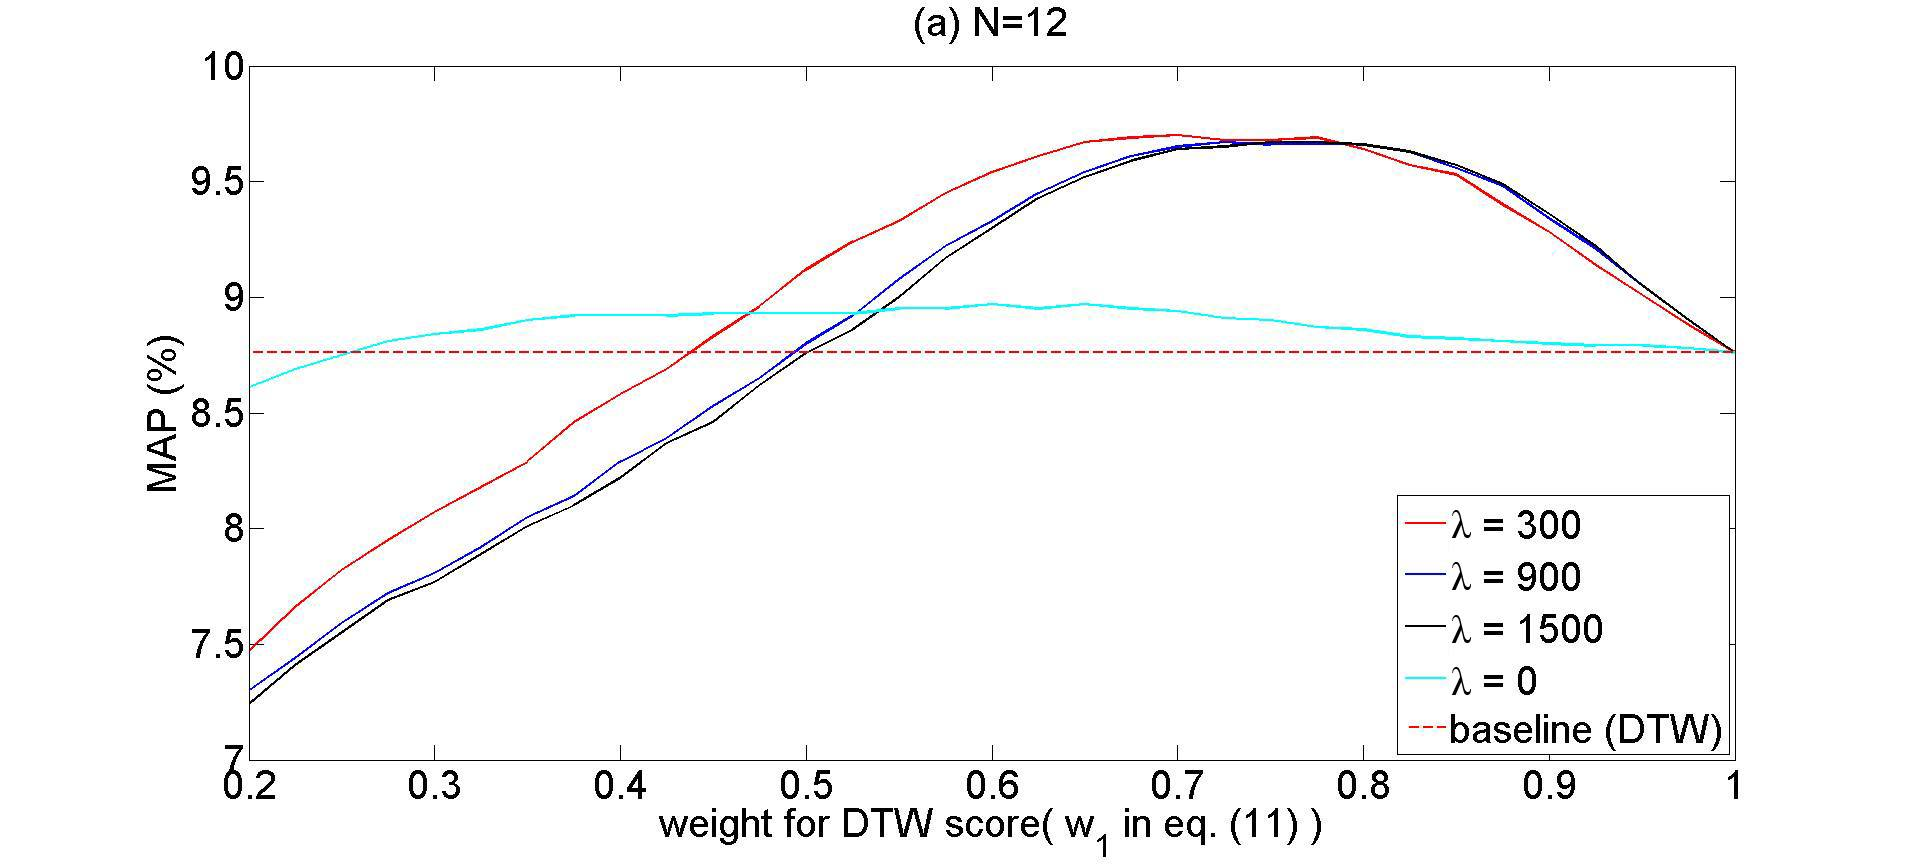
\includegraphics[scale=0.18]{images/chap4_resulta.jpg}
\caption{將第一次檢索結果和聲學組型形式的查詢詞擴展檢索結果疊加後的平均準確率 $(N = 800)$} \label{fig:chap4_resulta}
\centering
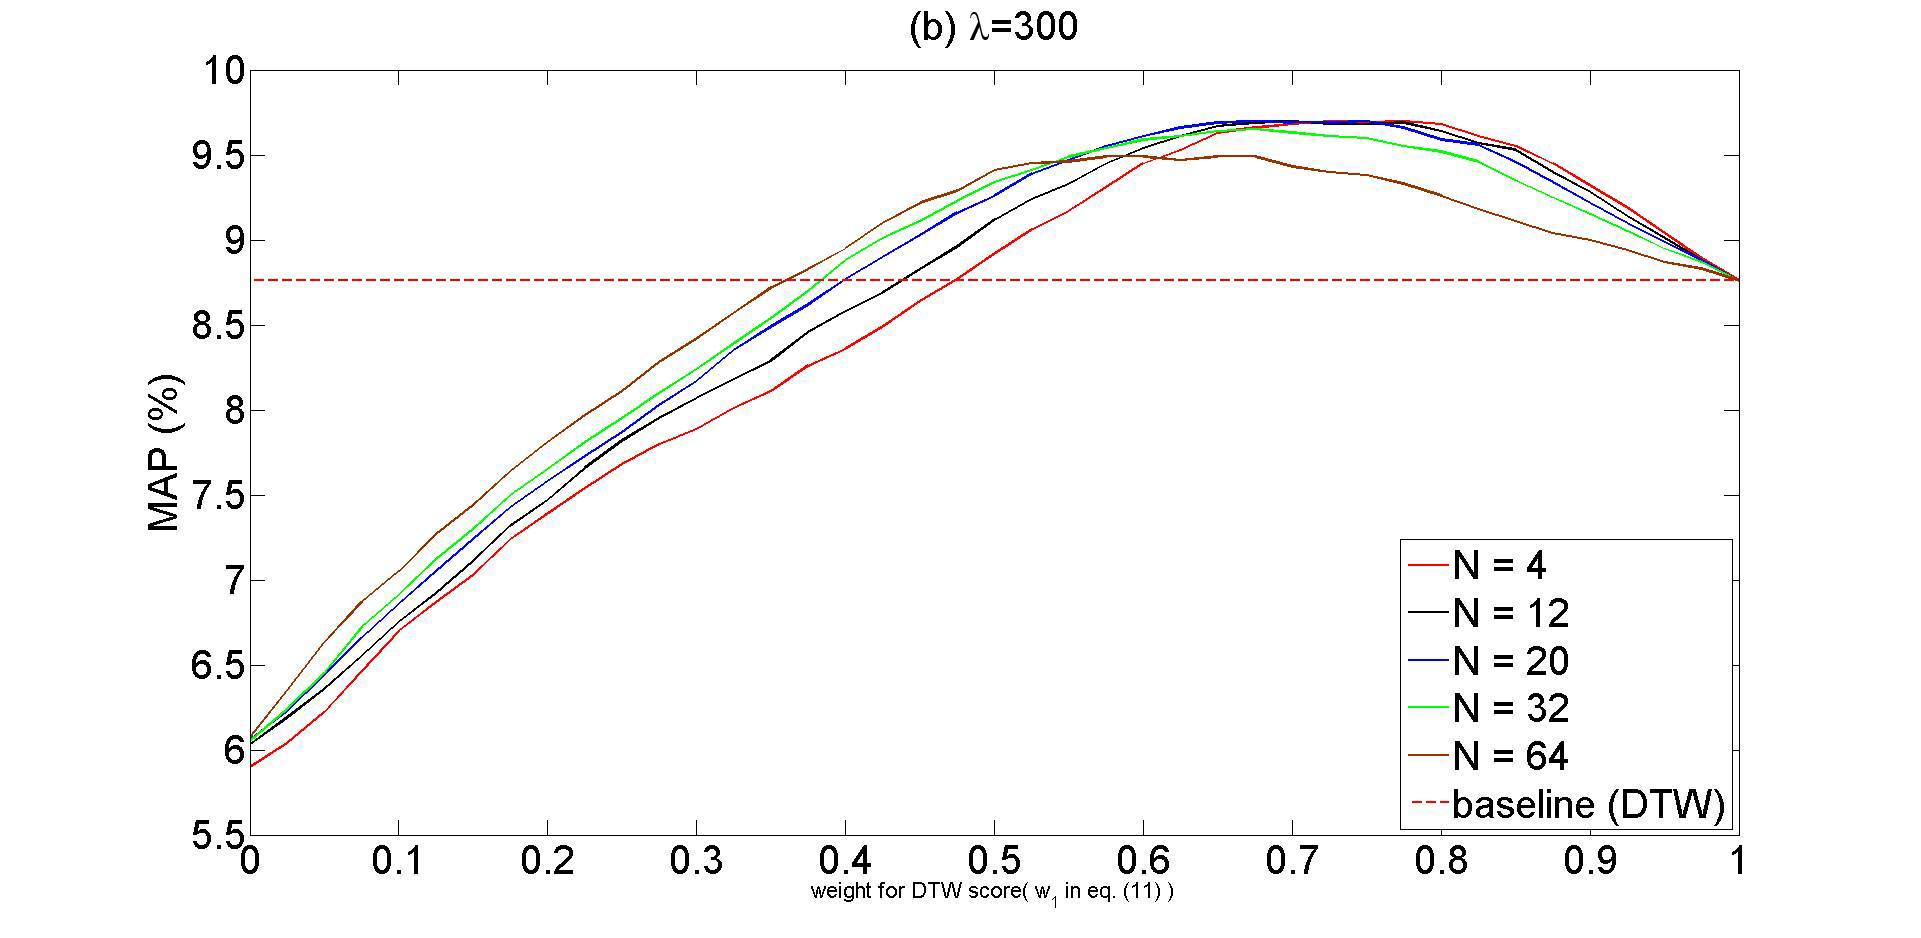
\includegraphics[scale=0.18]{images/chap4_resultb.jpg}
\caption{將第一次檢索結果和聲學組型形式的查詢詞擴展檢索結果疊加後的平均準確率 ($\lambda = 300$)} \label{fig:chap4_resultb}
\end{figure}


\subsection{聲學組型語意檢索能力分析}
表 ~\ref{table:chap4_spa} 中的實驗顯示了本章提出的方法確實能夠在聲學組型的查詢詞中加入與查詢詞語意相關的聲學組型,即使系統並不知道這些聲學組型的含義。表 ~\ref{table:chap4_spa} 中是「學校」這個查詢詞在經過本章的查詢詞擴展後機率 $P(v|\theta_Q)$ 最高的五個$N$連聲學組型 (由於聲學組型訓練時並沒有強制它一定是對應到中文的詞或是字,所以以下聲學組型對應到的聲音是經過很仔細的聆聽之後寫下它最接近的中文聲音)。列 (1)(2) 中的聲學組型為 ~\ref{sec:chap4_decode_query}
中提到的利用第一次檢索結果得到的原查詢詞的聲學組型,很明顯地列 (1)(2) 中的聲學組型在擴展後的查詢詞模型中也佔了大部分的機率。列 (3)(4)(5) 中的$N$連聲學組型則是在查詢詞擴展的過程中被自動加進去的,列 (3) 是由列 (1)(2) 中的單連聲學組型組合而成的雙連聲學組型,列 (4) 中的單連聲學組型對應到的中文聲音其實是與列 (2)
中非常相似,但由於訓練時因為聲學上的特徵不一樣而被分群為不同的聲學組型,在此本章的方法也能將這些片段加進來進而提升檢索結果。而列 (5) 加進來的是雙連聲學組型,當我們去聽這個聲學組型對應到的聲音時,發現聲音很像中文的「學生」,而這是與查詢詞「學校」有語意相關的詞,因此被系統加進來後也能提升檢索的結果。由以上的觀察可以發現本章提出的方法確實能把與查詢詞語意相關的聲學組型加進查詢詞模型中,並達成非監督式語意檢索。

\begin{table}[htbp]
\centering
%\resizebox{\columnwidth}{!}{     
\begin{tabular}{llll}
\hline
& $v$(n連聲學組型): (IDs) & $P(v|\theta_Q)$ & 聲學組型舉例 \\
\hline 
(1) & 單連: (87) & 0.4280 & 校(/xiao/) \\
(2) & 單連: (56) & 0.3880 & 學(/xue/) \\
(3) & 雙連: (56)-(87) & 0.0040 & 學校(/xue-xiao/) \\
(4) & 單連: (129) & 0.0030 & 學(/xue/) \\ 
(5) & 雙連: (129)-(23) & 0.0016 & 學生(/xue-sheng/) \\
\end{tabular}
%}
\caption{查詢詞為"學校(/xue-xiao/)"時,擴展後查詢詞模型 $\phi_{qe}$中機率最大的五組聲學組型}
\label{table:chap4_spa}
\end{table}

\section{本章總結}
本章嘗試了使用聲學組型完成了非監督式的語意檢索,使用此種方法即可在不需要人為標注的情況下達成語意檢索。如此一來即不需要花費很多時間、金錢完成人為標注,不過目前非監督式語意檢索的表現比起監督式仍有一段落差,仍然需要更多的研究才能夠使其應用在產業中。
